\section{结论与讨论}\label{sec:conclusion}

\begin{chapterquestion}
\textbf{本章研究的问题}：可信代理优化框架能带来哪些工程启示？
\end{chapterquestion}

\subsection{贡献与发现的区分}

本文区分\emph{贡献}（团队所做的工作：方法、流程、机制）
与\emph{发现}（团队得到的结论：规律、判断）。

\vspace{0.2cm}
\noindent\textbf{Contributions（贡献）}
\begin{enumerate}
    \item \textbf{受限算力下的代理模型驱动优化框架}：
        在 6 模型谱系中确立 XGBoost（可解释/公平比较）与 DeepEnsemble（提供 $\sigma$）双模型策略；
    \item \textbf{不确定性感知的可信优化机制}：
        以 $\mu(x)-\lambda\sigma(x)$ 风险敏感目标作为防御，
        OOD 压力测试表明其将越界率（$\mu>100$）从最高 $27.6\%$ 降至 $0\%$；
    \item \textbf{不确定性引导的数据精炼}：
        以局部重采样修补高不确定区域，支持认知盲区存在的判断（高不确定区 MSE $-55.9\%$）；
    \item \textbf{可信代理优化的诊断流程（核心贡献）}：
        构建并验证了
        "异常发现 $\to$ 不确定性分析 $\to$ 数据精炼 $\to$ 景观诊断 $\to$ 根因定位"
        这一可迁移的诊断流程；该流程本身是方法论产物，而非某个具体结论。
\end{enumerate}

\vspace{0.2cm}
\noindent\textbf{Key Finding（发现）}
\begin{chapterquestion}
\textbf{景观退化与数据结构限制，与优化结果趋同现象高度一致。}
在代理模型驱动优化中，数据覆盖度、不确定性管理与优化景观结构，
比优化器选择本身更决定最终优化质量。
\end{chapterquestion}

需要说明：景观诊断支撑了这一发现，但它是当前最有说服力的解释，
而非全文唯一支柱（见第~\ref{subsec:counterfactual}~小节）。

\vspace{0.2cm}
\noindent\textbf{方法边界与外部有效性}：上述\emph{发现}是在本数据集上得到的重要影响因素，
而非普适规律；本文真正可迁移的\emph{贡献}是诊断流程本身。
就课程定位而言，本研究的对象始终是代理模型驱动的智能优化问题：
PSO、GA、DE 与代理优化均属计算智能方法，
可信性分析是对计算智能优化系统的扩展研究，而非脱离课程主题的新课题。

\subsection{案例研究：Porpoising 风险空间刻画}

作为框架的应用案例（Case Study，对应框架的工程应用价值，不承担主线分析），
本文将框架用于海豚跳风险的空间刻画。

\begin{figure}[H]
\centering
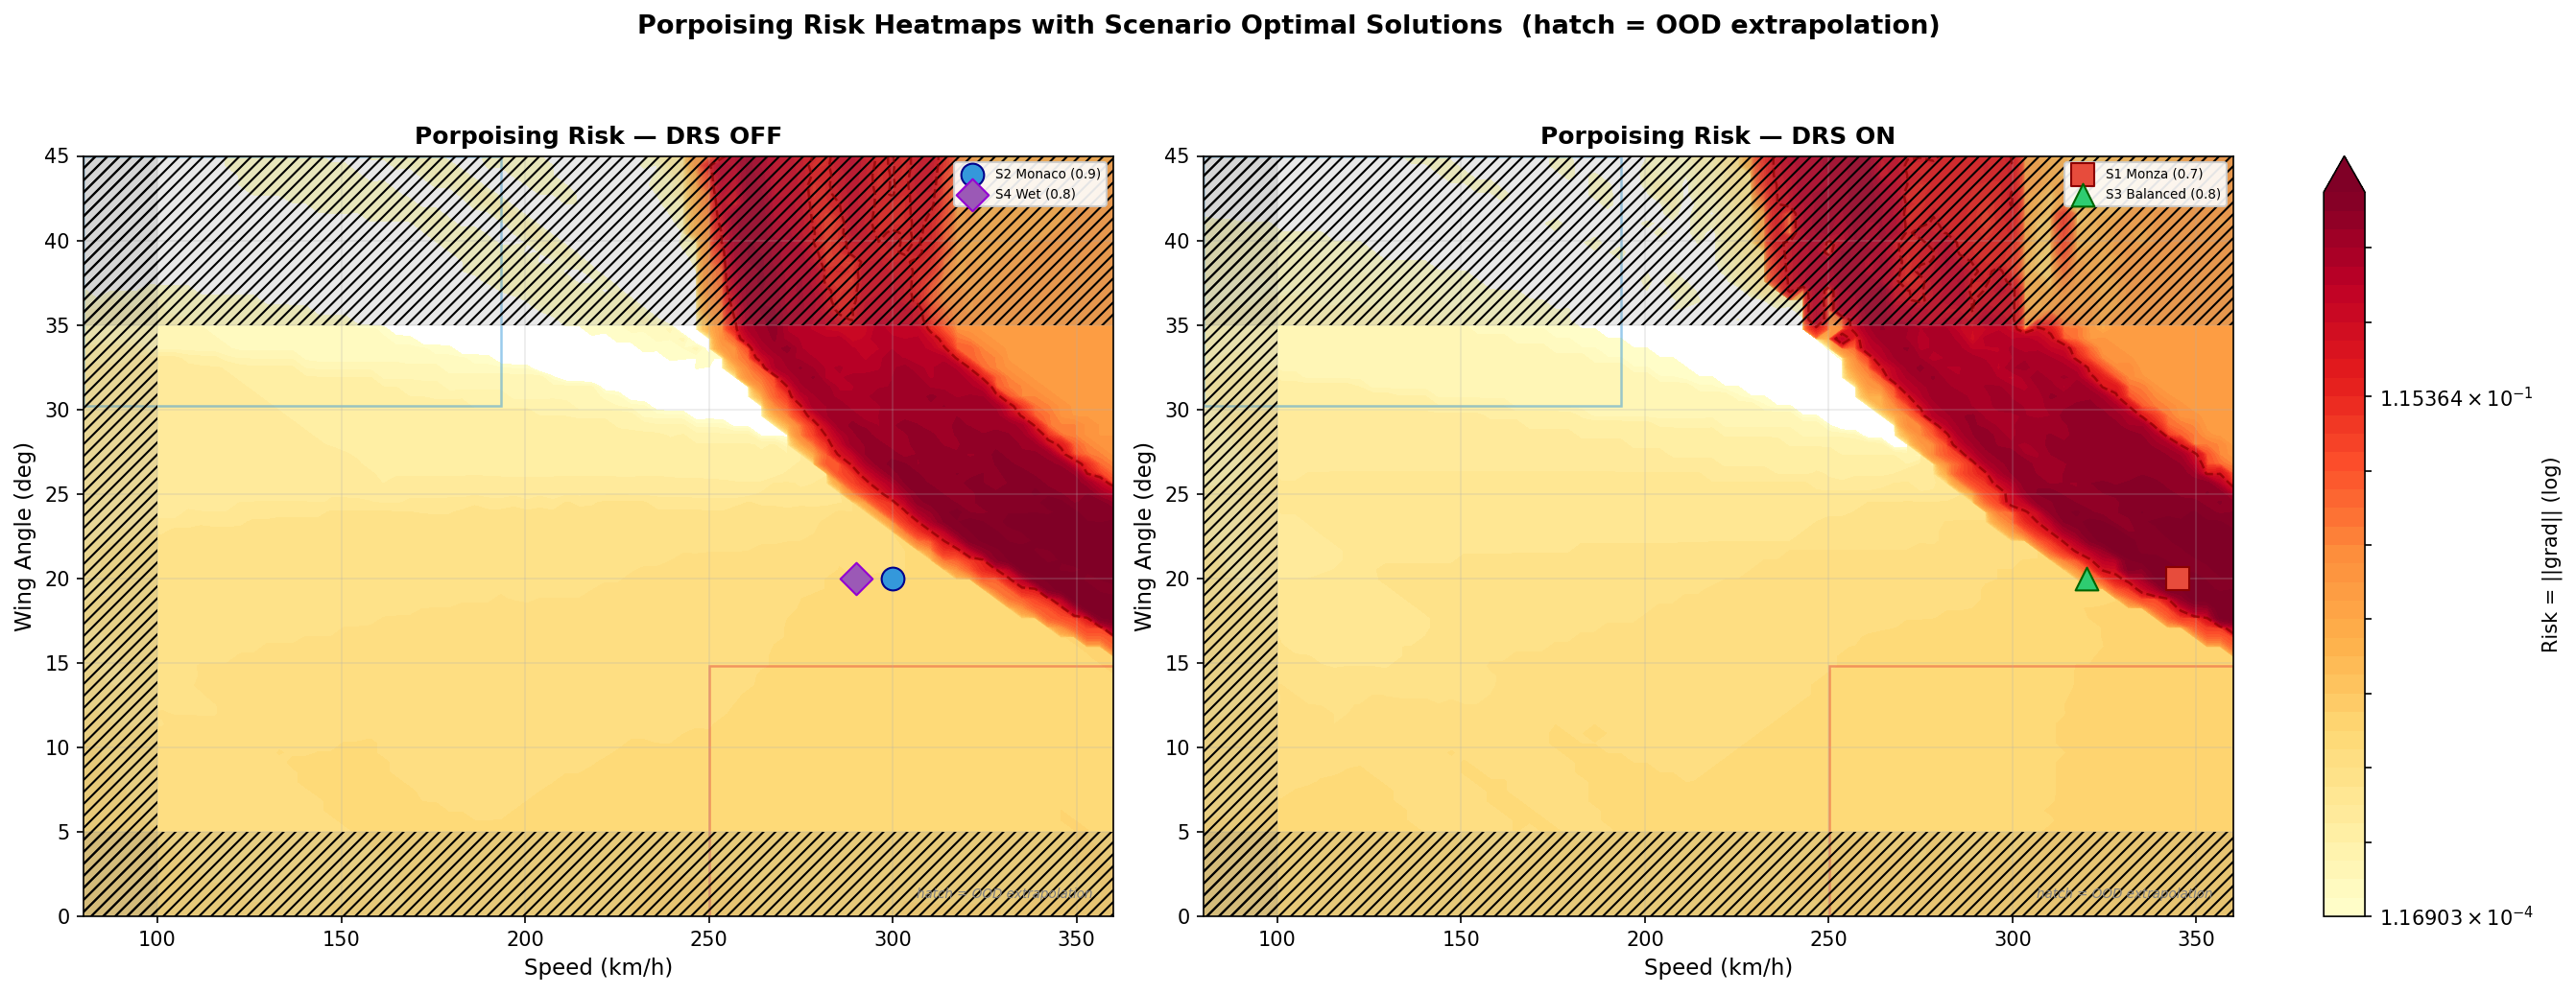
\includegraphics[width=0.85\textwidth]{figures/risk_vs_optimal_overlay.png}
\caption{风险热力图与多场景最优解叠加（DRS=0/1）}
\label{fig:risk_overlay}
\end{figure}

以 DeepEnsemble 梯度幅值 $\|\nabla f\|$ 作为海豚跳风险代理，
在 (speed, wing) 平面构建一阶风险热力图：高速$+$小翼角的 Zone A 风险约为
低速$+$大翼角 Zone B 的 $6.5$ 倍，与气动经验一致；
二阶 Hessian 分析显示高稳定区曲面极度平坦（约 $70\%$ 网格凹性但曲率幅度 $\approx0.03$），
与景观退化的判断一致。
图~\ref{fig:risk_overlay} 表明四场景最优解均位于低风险区，
从应用侧印证了风险敏感 PSO 的 OOD 回避行为。
需指出，该风险为代理梯度的间接估计，更直接的刻画需 CFD 或实验数据支撑。

\subsection{不足与局限}

\begin{enumerate}
    \item \textbf{数据非真实 CFD}：结论针对"代理驱动优化"这一方法论对象，不外推真实赛车；
    \item \textbf{同源与共线}：数据由 XGBoost Generator 生成、主代理同样采用 XGBoost，
        构成"XGBoost 学习 XGBoost"的同源结构，高 $R^2$ 受同源偏置影响、不证真实泛化；
        且 downforce$\leftrightarrow$drag 共线（$r=0.895$），使可解释性结论限于统计关联层面；
    \item \textbf{精炼仅单轮}：未形成多轮闭环，边际收益递减特性留待未来；
    \item \textbf{风险为间接量}：$\sigma(x)$ 是代理的不确定性，而非物理风险。
\end{enumerate}

\subsection{反事实稳健性分析}\label{subsec:counterfactual}

为避免将全文结论建立在单一根因之上，本节做一次反事实分析。
假设未来研究否定了"景观退化"的解释（不存在平台效应/梯度消失），
本文的主要结论是否仍然成立？

本文的多数实证基础不依赖景观结论：代理高精度、三类异常的观测事实、
$\sigma$ 度量的不确定性、数据精炼对盲区的修复、算法间同解（极差 0.15）均不受影响。
被否定的仅是"为何同解"的某一种机制性解释。
此时核心解释框架将由景观转向\textbf{数据覆盖问题}
（OOD 与不确定性是其表现形式）：解的趋同将被归因于优化被约束在
训练数据流形支撑的同一高置信区域内。
无论主要因素落在景观还是数据覆盖，本文主线依然成立——
这也是将贡献定义为"诊断流程"、将发现表述为"重要原因"（而非"唯一原因"）的用意。

\subsection{未来工作}

（1）物理信息代理模型，将气动平衡方程作为约束嵌入训练，以缓解目标饱和；
（2）多轮主动学习，刻画迭代精炼的边际收益递减特性；
（3）CFD-代理混合策略，以限量真实仿真替代检索式重采样；
（4）贝叶斯优化对比，用 DeepEnsemble 的 $\sigma(x)$ 构造采集函数，
与风险敏感 PSO 的可信优化行为进行对照。

\subsection{结语}

\begin{chapterquestion}
本文案例表明，代理模型的预测精度并不足以保证优化结果的可信性。
在代理驱动优化中，不确定性管理与数据覆盖分析应作为优化流程的重要组成部分。
\end{chapterquestion}
